\subsection{Adblock f�r Mozilla Firefox}
F�r Mozilla Firefox steht mit \textbf{Adblock Plus}\footnote{ \href{https://addons.mozilla.org/en-US/firefox/addon/adblock-plus/}{https://addons.mozilla.org/en-US/firefox/addon/adblock-plus/}} ein Add-on f�r das listenbasierte Blockieren von Werbung zur Verf�gung. F�r AdBlock Plus gibt es viele Listen zum Blockieren von Werbung (l�nderspezifisch), Tracking-Diensten und der Social Media Like-Buttons. Ein einfacher Klick auf das Install-Symbol der Website startet den Download der Erweiterungen und installiert sie.\\

Nach dem Neustart ist mindestens eine Filterliste zu abonnieren (Bild \ref{abb:adblock1}). Standardm��ig wird f�r deutsche Benutzer die Liste \textit{EasyList Germany + EasyList} vorgeschlagen. \textit{EasyList} ist eine gute Wahl, die man akzeptieren kann.

\begin{figure}[htb]
\begin{center}
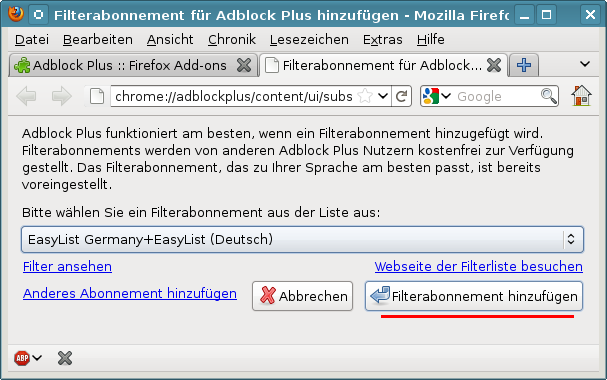
\includegraphics[scale=0.75]{../screenshots/adblock-firststart.png}
\caption{Auswahl einer Liste nach der Installition von Adblock Plus}
\label{abb:adblock1}
\end{center}
\end{figure}

\subsubsection*{Zus�tzliche Filterlisten abonnieren}
Weitere Filterlisten k�nnen im Einstellungen von AdBlock Plus unter dem Men�punkt \textit{Filter Preferences} abonniert werden. Hier ist der Men�punkt \textit{Filter -> Abonnement hinzuf�gen} zu w�hlen. Aus der Liste der angebotenen Filter k�nnen regional passende Listen gew�hlt werden. Folgende Filter-Listen sind als Erg�nzung zur EasyList passend:
\begin{itemize}
 \item \textbf{EasyPrivacy} blockiert meist unsichtbare Tracking-Elemente zum Aussp�hen ihres Verhaltens im Internet mit HTML-Wanzen. Die Liste ist eine sinnvolle Erg�nzung zur EasyList (Germany). Bei der Installation von \textit{EasyPrivacy} kann die zus�tzliche empfohlene EasyList deaktiviert werden, das sie bereits vorhanden ist.
 \item \textbf{SocialMediaBlock} ist eine Liste zum Blockieren der verschiedenen Social Media Tracking Features wie Facebook Like Buttons u.�. Zur Installation kopiert man folgende URL in die Adressleiste von Firefox: \href{abp://subscribe/?location=http://monzta.maltekraus.de/adblock\_social.txt\&title=SocialMediaBlock}{abp://subscribe/?location=http://monzta.maltekraus.de/adblock\_social.txt\&title=SocialMediaBlock}.
\end{itemize}

\subsubsection*{Whitelisting von Websites}
Mit der Version 2.0 hat AdBlock eine Whitelist f�r unaufdringliche Werbung eingef�hrt. Die Filterung wird auf den Webseiten in der Whitelist abgeschaltet, so dass diese Webseiten Werbung einblenden k�nnen. Bisher ist die Whitelist ziemlich leer. Man kann dieses Feature wie in Bild \ref{abb:adblock2} in der �bersicht der Filterlisten abschalten, indem man die Option \textit{Nicht aufdringliche Werbung zulassen} deaktiviert. Alternativ kann man auch das Add-on \textbf{TrueBlock} statt AdBlock verwenden. Es ist 100\% kompatibel mit AdBlock, das Whitelisting ist jedoch standardm��ig deaktiviert. \\

\begin{figure}[htb]
\begin{center}
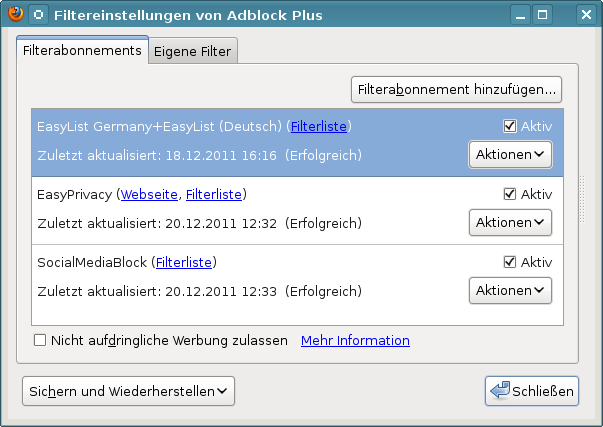
\includegraphics[scale=0.75]{../screenshots/adblock-whitelist.png}
\caption{Whitelisting in AdBlock Plus deaktivieren}
\label{abb:adblock2}
\end{center}
\end{figure}

Statt dessen kann man selbst entscheiden, welchen Webseiten man das Anzeigen von Werbung gestatten m�chte. Mit einem gelegentlichen Klick auf Werbung kann man gute Webseiten bei der Finanzierung unterst�tzen. Wenn Sie eine Webseite im Browser ge�ffnet haben, k�nnen Sie in den Men� von AdBlock die aktuelle Webseite zu einer eigenen Whitelist hinzuf�gen.

\subsubsection*{Vertipper korrigieren}
Die Entwickler von AdBlock sind der Meinung, dass das Korrigieren von Vertippern in der URL ein sinnvolles Feature f�r einen Werbeblocker ist, und haben \textit{URL Fixer} integriert. Die Tippfehlern werden an den Server \textit{urlfixer.org} gesendet und dort gesammelt. Es wird vielen Nutzern nicht gefallen, wenn Daten �ber gerade besuchte Seiten an einen externen Server gesendet werden. Einen Hinweis auf die Daten�bertragung findet man nicht.\\

Man kann dieses (�berfl�ssige) Feature in den Filtereinstellungen von AdBlock auf dem Reiter \textit{Vertipper-Korrekturen} deaktivieren. 

\subsubsection*{Anti-AdBlock}
Anti-AdBlock ist ein Script f�r Webmaster, die den Besucher der Webseite zur Deaktivierung von AdBlock Plus zwingen wollen. Bei aktivem Werbeblocker sieht man beim Besuch einer pr�parierten Webseite nur folgenden Hinweis: 
\begin{center}
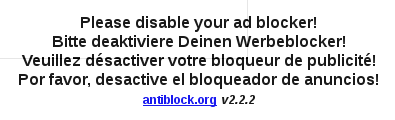
\includegraphics[scale=0.7]{../screenshots/anti-adblock.png}
\end{center}
Wer sich nicht g�ngeln lassen will, kann das Firefox Add-on \textbf{Disable Anti-Adblock}\footnote{ \href{https://addons.mozilla.org/en-US/firefox/addon/disable-anti-adblock/}{https://addons.mozilla.org/en-US/firefox/addon/disable-anti-adblock/}} installieren. Dann kann man die Webseite werbefrei betrachten. 
